% dev_guide.tex

\documentclass{book}
\usepackage{times}
\usepackage{alltt}
\usepackage{graphicx}

\begin{document}

\title{ Oxide Developer's Guide }
\author{ Samuel Mulder }
\date{\today}
\maketitle

\chapter{System Overview}

\section{Introduction}
Oxide is a flexible, modular, distributed framework for performing analysis of executable code.  It separates the user interface components from the storage components and from the analysis components.  For example, Oxide has several interface scripts that may be used to drive the system, two different back-ends that may be used for storage, and many analysis modules.  The system is designed such that a module writer who is a domain expert in the specific area of the module does not need much knowledge of the rest of the system.  The same modules work no matter how or where the data is stored or what sort of interface the user is seeing.  In addition, the Oxide system handles auto dependency resolution, so a module writer who is a domain expert in clustering techniques and wants to work with opcode ngrams for example does not have to have any knowledge of the disassembly chain or other complexities involved in producing the desired ngrams. 

\section{Code Analysis}
\begin{figure}
\centering
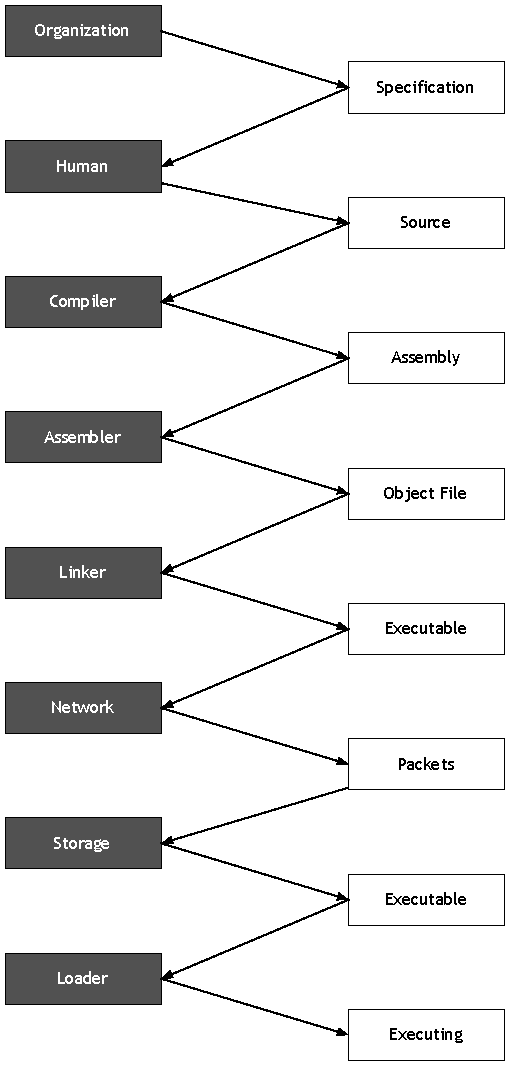
\includegraphics[width=0.6\textwidth]{pdf/provenance.pdf}
\caption{Code Provenance}
\label{provenance}
\end{figure}

The analysis of executable code is challenging because the final artifacts that are discovered have been through multiple layers of translation from the original sources that we are interested in, see Figure~\ref{provenance}.  We may care about the organization sponsoring malware, or the individual author who wrote the code, or the functionality.  We typically have access to either an executable file on disk or a packet stream containing the file in question.  To unravel the complexity of the final software, Oxide uses a layered, modular approach to feature extraction (Figure~\ref{oxide-modules}).

\begin{figure}
\centering
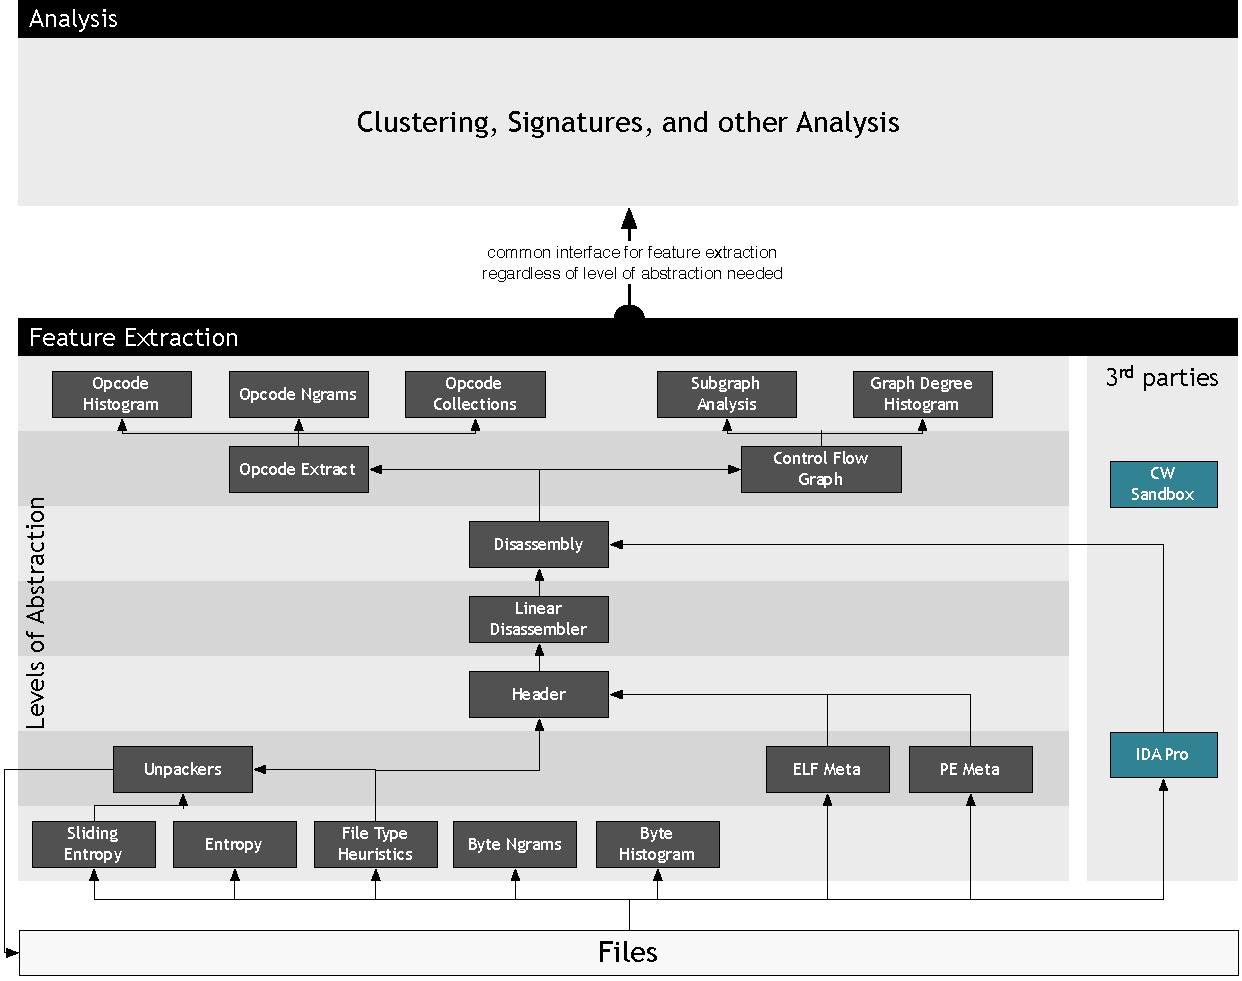
\includegraphics[width=1.2\textwidth]{pdf/modules.pdf}
\caption{Example modules in Oxide}
\label{oxide-modules}
\end{figure}


\chapter{API}
All scripts and modules that are part of Oxide or use Oxide, should import api.  The following functions are provided by the Oxide system.

\subsubsection{store(mod\_name, oid, data, opts=None)}

The store function is used by modules that store results.  All extractor modules should call this if valid features are extracted.  The parameters are the module name, the oid that you wish to use as a key, the data to store (this should always be a dict), and the options dictionary that the module was called with.  If your module has no mangle options, you can leave off the opts dict as it is used to create a unique key for different values of the mangle options.  This function returns a boolean to indicate success or failure.

\subsubsection{source(oid)}

The source function is used to determine the source module for a given oid.  Unless you are using specialized source modules, this will generally be either "files" or "collections".  This should always be used instead of making the assumption that a given oid belongs to a file.  The return value is the module name of the source module.
                
\subsubsection{process(mod\_name, oid\_list, opts=None)}

The process function is used to call modules if you do not want the results returned immediately.  It does not necessarily cause the module to execute if the module has already been run over the given oid and there are no mangle options.  A boolean return value indicates whether the process was either run successfully or already existed (True) or whether there was some problem or error (False).  The oid\_list may be either a single oid or a list of oids.  How it is handled depends on the module type.
               
\subsubsection{exists(mod\_name, oid, opts=None)}

The exists function returns a boolean indicating whether the module name - oid combination exists in the datastore.  If options are specified then it will take mangle options into account.                

\subsubsection{retrieve(mod\_name, oid\_list, opts=None)}

Retrieve is the way to get the result of any module.  If the analysis already exists, then it will be retrieved from the datastore directly.  Otherwise, the module will be run to generate it.  Note that this means that a given module may or may not be called depending on the state of the datastore.  Never directly index into the returned dictionary without validating that the desired key exists.

\subsubsection{get\_field(mod\_name, oid, field, opts=None)}

This is the preferred way to retrieve data if only a single field is needed from another module.  The field specified should be a key in the dictionary saved out by the given module.  This function has the advantage of doing validation and will return None if the field does not exist.  Always test for a None result.
             
\subsubsection{expand\_oids(oids)}

Expand\_oids takes either a list of oids or a single oid and walks through expanding any set types (ie collections) into the constituent atomic oids.  This is useful if you want to receive sets of oids but can only process each one atomically.  This is called internally, for example, in the case where process is called with a collection id on a module that only handles atomic ids.  A list of the expanded ids is returned.

\subsubsection{get\_oids\_with\_name(some\_name)}

This function searches through all of the source modules and examines the "names" field for a match.  It returns a dictionary of oids where the value indicates the source type.  This should be used cautiously as oids in the system may be associated with multiple names and any name may be associated with multiple oids.
    
\subsubsection{get\_colname\_from\_oid(oid)}

This function returns the name of a collection with the given oid

\subsubsection{get\_names\_from\_oid(oid)}

This is a mirror of the previous function.  The return value is a set of names associated with the oid.  Since a given oid should only every have one source, use the source function to get the source.  Some oids may not have a name associated with them.  There are several possible reasons for this depending on the way the oid was generated.  Some source modules (e.g. chunks) do not generate a name. 

\subsubsection{get\_oid\_from\_data(data)}

This function is the canonical way to generate oids in the system.  It takes a string and calculates a sha1 hash that is returned as the oid.  This should always be used instead of calculating the hash directly so that a different hash function may be substituted in future versions.
     
\subsubsection{create\_collection(col\_name, oid\_list, notes)}

This function is used to create a collection from a list of oids.  The oid list should include only atomic oids, i.e. not other collections.  It will return a boolean indicating whether the collection was created.  If the collection name is already in use or if an identical collection with a different name exists then the function will fail.  This should be used sparingly.  It is preferable to allow the user to create collections explicitly.

\subsubsection{scratch\_dir}           

This is not a function, but a string that is the absolute path of the scratch directory to be used by Oxide.  Always use this instead of writing to a module directory or some other location for temporary files.  Modules should never directly interact with the filesystem except through this directory.

\subsubsection{models\_dir}           
This is not a function, but a string that is the absolute path of the models directory to be used by Oxide. 

\subsubsection{documentation(mod\_name)}

This function returns the documentation dictionary for a module.  It may be used to verify properties of modules before calling them.  An example use case is a script or module that allows a module name to be passed in as an option and then calls that module.  See the section on writing modules for the format of this dictionary.

\subsubsection{get\_cid\_from\_name(col\_name)}

This function takes a name of a collection and returns the oid of that collection if it exists or None if it does not.
    
\subsubsection{modules\_list(mod\_type="all", show\_private=True)}

The default state of this function is useful for determining whether a module exists in Oxide, e.g. for validating a parameter passed in that is supposed to be a valid module name.  It can also be used with alternate parameters in scripts that wish to display modules to the user interface.  The return value is a list of module names.  Valid mod\_type values are "all", "source", "extractors", "analyzers", and "map\_reducers".  Show\_private indicates whether private modules should be returned and is mostly useful in user interface scenarios.         

\subsubsection{import\_file(file\_location)}

This function is used to import a new file into Oxide.  It returns a tuple consisting of the oid of the file in the system (or None if it failed), and a boolean indicating whether the file was new to the system or already existed.

\subsubsection{import\_directory(directory\_location)}

This function is used to import an entire directory into Oxide.  It returns a tuple consisting of a list of oids of the files in the directory (or None if it failed), and an integer count of the number of files new to the system.
          
\subsubsection{apply\_tags(oid\_list, new\_tags)}

This function applies the set of tags specified to each oid in the oid\_list.  The new tags should be passed in as a dictionary with tag names as keys and associated values. 
          
\subsubsection{get\_tags(oid)}

This function returns the dictionary of tags currently applied to the given oid.

\subsubsection{tag\_filter(oid\_list, tag, value)}

This functions returns a filtered subset of oids from the oid\_list (or from all oids in the files module if None is passed in as the oid\_list).  If you just want to filter on the existance of a tag, then pass a value of "<empty>".

\subsubsection{retrieve\_all\_keys(mod\_name)}

This function returns a list of all oids that have been stored by the given module.  If the module has never been run or does not store out, then this will be an empty list.

\subsubsection{collection\_names()}

This function returns a list of all collection names currently in the datastore.

\subsubsection{collection\_cids()}

This function returns a list of all collection oids currently in the datastore.

\subsubsection{get\_cid\_from\_oid\_list(oid\_list)}

This function takes a hash of the given oid\_list after deduping and ordering that may be used as the collection id.

\subsubsection{valid\_oids(oid\_list)}

This function returns a tuple of two lists, usually named (valid, invalid).  The first list consists of oids that exist in the system and the second of anything else in the original oid\_list.  This is frequently used by plugins to filter their input and make sure they only try to retrieve results from valid oids.

\subsubsection{flush\_oid(oid)}

The function flush\_oid deletes all stored data from any module that is associated with an oid.

\subsubsection{flush\_module(module)}

The function flush\_module deletes all data associated with a particular module.

\subsubsection{local\_store(function\_name, data\_name, data)}

The local\_store function is used by plugins to store results locally. The parameters are the function name, the name of the data and the, the data to store which should always be a dict. This function returns a boolean to indicate success or failure.

\subsubsection{local\_exists(function\_name, data\_name)}

The local\_exists function returns a boolean indicating whether the function name - data name combination exists in the local storage.

\subsubsection{local\_retrieve(function\_name, data\_name)}

The local\_retrieve function is the way to get the locally stored results of any function. 

\subsubsection{local\_available\_data(function\_name)}

The local\_available\_data function returns a list of locally stored data names associated with a function.

\subsubsection{local\_retrieve\_all(function\_name)}

The local\_retrieve\_all function returns a dictionary of locally all stored data associated with a function. The keys of the dictionary are the data names and the values of the dictionary are the data

\subsubsection{local\_count\_records(function\_name)}

The local\_count\_records fuction return the number of locally stored data files associated with a particular function.

\subsubsection{local\_delete\_function\_data(function\_name)}

The function local\_delete\_function deletes all locally stored data associated with a particular function.

\subsubsection{local\_delete\_data(function\_name, data\_name)}

The local\_delete\_data function deletes locally stored named data associated with a functions.

\chapter{Plugins}
Chunks of functionality that do not store into the datastore and benefit from chaining interatively with other plugins, should be written as a plugin.  In distributed environments, plugins will always run on the same machine as the shell.  For this reason, they should only interact with the rest of the system through the API. Plugins have the advantage that they are loaded dynamically and so do not clutter the namespace when in use.

A plugin should be written as a python source file and saved in  
\begin{verbatim}\plugins
\end{verbatim} 
A plugin should contain a global list called exports that contains the functions intended to be exposed to the shell.  It is convenient to place these functions first in the file and place other utility functions later in the file.  All exported functions must be of the form:
\begin{verbatim}def plugin_name(args, opts):
\end{verbatim}
The args list that comes in will be a combination of items specified on the call line followed by things piped in from previous commands in the chain.  The shell handles option parsing and the opts dictionary will contain key, value pairs as specified on the command line with --key=value. 

For example, the following line:
\begin{verbatim}&test | my_plugin %a123412225ab341 --verbose --n=3
\end{verbatim}
will result in my\_plugin being called where args is a list consisting first of the oid a123412225ab341 followed by the oids in the collection test.  The opts dictionary will contain \{ "verbose":None, "n":3 \}

Plugins should always return a list containing some result, or an empty list if nothing makes sense.

Disadvantages to writing plugins are that they are not parallelized or distributed by the system, they may not be dependencies of modules, and any data retrieved from the datastore may have to pass over the network in a remote environment.  The main advantage is that they may be chained dynamically in the shell, display output to the screen, and are fairly unconstrained with respect to functionality.

Conventions for plugins are still in the process of being established and so remain fluid.  A common convention is to accept a list of oids, do some processing and return a list of oids.  Other plugins are primarily intended for displaying or outputting data and so are not as concerned about returning data.  Always try to consider how your plugin could be usefully chained together with other plugins.  Consider returning something that is useful for the show plugin rather than printing directly, etc. 

\chapter{Modules}
Functionality that caches to the datastore or needs to be run on the same machine as the datastore should be written as a module.  Every module in the system should exist in its own directory in the appropriate subdirectory under the modules directory in Oxide.  Under the main Oxide directory, the following directory tree contains all of the modules in Oxide:
\begin{verbatim}\modules
        __init__.py
        /analyzers
                /module1
                /module2
                ...
        /analyzers_dev
                /module3
                /module4 
                ...
        /extractors
                /module5
                /module6
                ...
        /extractors_dev
                ...
        /map_reducers
                ...
        /map_reducers_dev
                ...
        /source
                ...
        /source_dev
                ...
\end{verbatim}

There are four basic types of modules, and each module type has available a release and dev directory.  The availability of dev level modules to oxide users is controlled through the configuration file as described in the User Guide.  The four types of modules are source, extractor, analyzer, and map\_reducer. 

The first thing to do when creating a new module is to decide what type it should be.  Source modules are a special type that is used to create new IDs in the system.  In general, source modules should only be written by advanced developers who understand all of the ramifications of creating new IDs.  Most modules will be of the other three types.

Extractor modules are the simplest module type.  They take exactly one ID, retrieve information about that ID, generate (extract) some new feature associated with that ID, and store it out.  Extractor modules are highly constrained in the way they operate.  This has the benefit of guaranteeing that they are embarrassingly parallel and may be distributed freely in a distributed instance of the Oxide system.  If a module can fit this paradigm, then this is the recommended type of module.

Map\_reducer modules follow the Map-Reduce model.  They are commonly used for modules that operate on collections or groups of IDs and can be broken into two parts.  The first part maps a function over each ID and the second function collects the results of this mapping the performs some reduce operation that combines the results.  

Analyzer modules are the least constrained module type.  The advantage is that the module developer has a lot of flexibility.  They can accept a list of IDs, can choose to store results or not, and return some value directly to the system.  The disadvantage of analyzers is that the system can make no assumptions about parallelizing them and so must run them in a single process.  This has serious performance implications and analyzers should only be used where no other module type is appropriate.

The rest of the chapter will go into some detail about how to write a module.  The first sections will describe features that are applicable to all module types and further sections will describe features specific to each of the four module types.  The last section will include examples of each type of module.  
	
\section{module\_interface.py}

Every module must contain at least two files.  The first is an empty file named \emph{\_\_init\_\_.py} which allows the module to be imported into Oxide.  The second required file should be named \emph{module\_interface.py}.  This section describes the contents of the module interface.

Every module interface should begin with string definitions for \emph{desc} and \emph{name}.  The \emph{desc} string should be a short description of the module that will be used in interface menus and help.  The \emph{name} string should be the name of the module and it must be identical to the directory name containing the module.

The next few lines should include the imports for the modules.  In general, all modules should import at least \emph{logging} and \emph{api}.  

\subsection{Logging}
The logging import is the Python standard library logging module.  This can be imported and will inherit the configuration that Oxide has already set up for it.  
Modules should then include the lines:
\begin{verbatim}
logger = logging.getLogger(name)
logger.debug("init") 
\end{verbatim}
This insures that logging messages will be associated with the appropriate module name.  It also prints a standard message letting users debugging Oxide know that the module loaded.

Logging should be the only means of external communication, e.g. no prints should be used in modules.  This allows the end user or application scripts to manage this information and present it at the appropriate level.  

Modules should use the following guidelines for logging:

\begin{itemize}
\item \emph{logger.debug()} - used for normal status, signaling the start of functions, etc
\item \emph{logger.info()} - used to present information about processing in progress that is not critical, e.g. processing 12 files in this collection
\item \emph{logger.warning()} - used to present information about processing that may be important but doesn't prevent the module from running, e.g. recognition of a malformed header
\item \emph{logger.error()} - used to notify the user that some condition has prevented a module from running correctly, however the module should not crash
\item \emph{logger.critical()} - used to notify the user that the system is in a bad state and is exiting
\end{itemize}

\subsection{API usage}
The api import is an Oxide specific interface that gives the module developer access to features of Oxide.  This interface is the \textbf{only} way that a module should interact with the Oxide system.  Modules should never attempt to directly import or call other components and should not presume to know anything about the directory structure, datastore structure, etc. above their module directory.  Ignoring this guideline may lead to incompatibility and strange errors in configurations of the system that differ from the module developer's.
The most commonly used functions in the api will be \emph{api.get\_field()} and \emph{api.store()}.  These allow the module to retrieve analysis from other modules, including the raw data of the file, and to store out the results generated if required.  Please refer to the API section of this document for full documentation of all functions available in the api.

\subsection{opts\_doc}
The next line in the module interface should be the opts\_doc definition.  In many modules, this will be an empty dictionary.  If options are required, they must be specified in the following format.

The \emph{opts\_doc} is a dictionary where the keys are the names of each option and the values are a dictionary defining how that option is to be treated.  Parameters for each option include:

\begin{itemize} \item \emph{type} - The value should be the type expected.  This will be enforced in core and should not need to be validated in the module.  Constraints beyond type may still need to be validated.
\item \emph{mangle} - The value should be \emph{True} or \emph{False} and indicates whether differing values for this option will represent unique entries in the datastore.  For most options this should be \emph{False}.
\item \emph{default} - The value should be of the same type specified in \emph{type} and should contain the value to use if none is specified.  If you set this to \emph{None}, then the core will ensure that it is required to be specified.
\end{itemize}

As an example, the option doc for the \emph{file\_meta} module is:
\begin{verbatim}
opts_doc = {"file_location":
                {"type":str,  "mangle":False, "default":None},
            "stat":
                {"type":dict, "mangle":False, "default":None}}
\end{verbatim}

\subsection{documentation()}
After specifying the \emph{opts\_doc}, the module interface should define the documentation function.  This function accepts no parameters and returns a dictionary with the following entries.

\begin{itemize} \item \emph{description} - The value should be the \emph{desc} string described previously.
\item \emph{opts\_doc} - The value should be the \emph{opts\_doc}  described previously.
\item \emph{set} - The value should be \emph{True} or \emph{False} to indicate whether the module can accept set IDs, i.e. collections.  Setting this to \emph{False} for extractor modules causes the core to automatically expand the set ID and map the module over the constituent IDs.
\item \emph{atomic} - The value should be \emph{True} or \emph{False} to indicate whether the module can accept non-set IDs. e.g. files.
\item \emph{private} - This key is optional and if present should be set to \emph{True} and indicates that the module should not show up in default lists of modules to the user.  This is useful if it is a utility module that is only used by other modules or the shell.  If a module is not private, the key should not be present.
\end{itemize}
An example of the documentation function from the \emph{file\_meta} module is:
\begin{verbatim}
def documentation():
    return { "description":desc, "opts_doc":opts_doc, 
             "private":True, "set":False, "atomic":True}
\end{verbatim}

\subsection{Type-specific functions}
The remainder of the module interface varies depending on the type of the module.  Extractor and Source modules provide a \emph{process} function.  Map-Reducing modules provide a \emph{mapper} and a \emph{reducer} function.  Analysis modules provide a \emph{results} function.  The following sections describe the requirements of each of these functions.

\subsubsection{Extractor and Source modules}
Extractor and Source modules must implement the \emph{process()} function.  This purpose of this function is to take one ID and a dictionary of options, generate some new metadata which gets stored out, and then return True or False based on success or failure.  Typically, this function will begin with a call to \emph{api.get\_field()} to get either the raw file data or some previously generated metadata.  Then some processing will occur to generate some new data.  The function generally ends with a call to \emph{api.store()} and \emph{return True}.  

It should be noted that extractor modules do not return anything.  The metadata generated by an extractor can be accessed by scripts or other modules using the \emph{api.retrieve()} function.  These module types will be short-circuited by the system if the processing has already been done.  If the result is already in the datastore, the module's code will not be called.

\subsubsection{Example Extractor - elf/module\_interface.py}
\begin{verbatim}

desc = " This module uses the pyelf package to extract features from the ELF header."
name = "elf"

import logging
from interpret_elf import elf_repr
import api

# Standard logging initialization allows developers to see which
# modules produced log messages
logger = logging.getLogger(name)
logger.debug("init")

# This module has no options
opts_doc = {}

def documentation():
    return {"description":desc, "opts_doc":opts_doc, "set":False, "atomic":True }

def process(oid, opts):
    logger.debug("process()")
    src_type = api.get_field("src_type", oid, "type")
    if src_type != "ELF":
        return False
    file_data = api.get_field(api.source(oid), oid, "data")
    if not file_data:
        return False
    api.store(name, oid, {"header":elf_repr(file_data)}, opts)
    return True
\end{verbatim}

\subsubsection{Map-Reducing modules}
Map-Reducing modules must implement two additional functions, \emph{mapper()} and \emph{reducer()}.  The functions essentially implement the standard map-reduce algorithm, with the limitation that intermediate reducers are not available.  Map-reduce calls will never be short-circuited.  If short-circuit behavior is desired, it can be done manually, see the second example below.

The \emph{mapper()} function will be called for each ID in the set that is being processed.  This function has the option to \emph{api.store()} out intermediate results for individual IDs if this makes sense.  The function returns some intermediate result, which in many cases will be the IDs of files that matched some condition.  This intermediate value will be propagated to the \emph{reducer()} function.

The \emph{reducer()} function accepts a list of all intermediate results along with a \emph{jobid} that can be used to reference the full set.  In cases of a collection, the jobid will be the collection ID.  In other cases, an ID is generated by the core.  The \emph{reducer()} function may store out results when this makes sense.  It is required to return the results of the full map-reduce operation as a Python dictionary.  In the case of a failed run or no valid result, the function may return a \emph{None} value.

\subsubsection{Example Map-Reducer - byte\_histogram/module\_interface.py}
\begin{verbatim}
desc = " This module produces a histogram of "\
           + "the bytes in a file." 
name = "byte_histogram"        

import logging
from collections import defaultdict

# import functions from the histogram utility file
# this file is located in /core/libraries
# but is exposed by the Oxide system to modules
from histogram import build_histo, merge_histo
import api

# Standard logging initialization allows developers to see which
# modules produced log messages
logger = logging.getLogger(name)
logger.debug("init")

# This module has no options
opts_doc = {} 
   
def documentation():
    return {"description":desc, "opts_doc":opts_doc, 
              "set":False, "atomic":True }

# This module stores analysis out and short 
# circuits if the analysis already exists.
# This is done for you with extractors, but has
# to be manually handled with map-reducers.
def mapper(oid, opts, jobid=False):
    logger.debug("mapper()")
    src = api.source(oid)
    if api.exists(name, oid, opts):
        return oid
    data = api.get_field(src, oid, "data")
    if not data:
        return None
    out_histo = build_histo(data)
    api.store(name, oid, out_histo, opts)
    return oid

# The intermediate_output will be a list of all
# the values returned from the mappers, in this case
# the oids.        
def reducer(intermediate_output, opts, jobid):
    logger.debug("reducer()")
    out_histo = defaultdict(int)

    for oid in intermediate_output:
        if oid:
            histo = api.retrieve(name, oid, opts)
            out_histo = merge_histo(histo, out_histo)
    api.store(name, jobid, out_histo, opts)
    
    return out_histo          
\end{verbatim}

\subsubsection{Analyzer modules}
Analyzer modules are the least constrained module type.  They must implement the \emph{results} function.  This function accepts a list of IDs, which may be any combination of items.  No constraints are checked or enforced by the core, so care must be taken to call these correctly.  Analysis modules may store out values in the same way as other modules if desired, but will never be short-circuited.  The \emph{results} function must return the result of the analysis as a Python dictionary.  In the case of a failed run or no valid result, the function may return a \emph{None} value.

\subsubsection{Example Analyzer - disassembly/module\_interface.py}
\begin{verbatim}
desc = 'This module should be used by higher level '\ 
          +'modules that want to get disassembly.'
name = 'disassembly'

import api
import logging

# Standard logging initialization allows developers to see which
# modules produced log messages
logger = logging.getLogger(name)
logger.debug('init')

# choices is a list of possible valid extractor modules to pull from
choices = ['auto', 'linear_disassembler', 'ida', 'distorm_disassembler']

# This is a fairly typical opts_doc with one option
# The 'valid' key is optional and allows the shell to provide better
# feedback to the user.
opts_doc = {'module': {'type': str, 'mangle': False, 'default': 'auto', 
            'valid': choices}}

def documentation():
    return {'description': desc, 'opts_doc': opts_doc, 
	     'set': False, 'atomic': True}

def results(oid_list, opts):
    logger.debug('results()')

    # The choose_disassembler function makes sure that the module
    # option is valid or if it is auto tries to determine the 
    # best disassembler to call out to.
    disassembler = choose_disassembler(opts)
    if disassembler not in choices:
        logger.warn('disassembly only accepts (%r)' % choices)
        return None

    # Since this is indirectly calling 3rd party code, it catches 
    # exceptions and just returns none so that it will fail gracefully.  
    # This makes it hard to debug code covered by this, 
    # but makes the system more robust.
    try:
        disasm = api.retrieve(disassembler, oid_list[0], {})

    except Exception, msg:
        logger.error("disassembly failed for %s: %s", oid_list[0], msg)
        return None

    return disasm
\end{verbatim}

\section{Code Conventions}
There are some basic guidelines that need to be followed to keep the system consistent and make sure that things stay sane even when combinations of modules never envisioned by the original authors are strung together.
\begin{itemize}
	\item The \emph{process()} function should always return only \emph{True} or \emph{False}.
	\item The \emph{results()} and \emph{reducer()} functions should always return either a \emph{None} or a Python dictionary with consistent keys.
	\item No module should ever throw an exception.  If using a 3rd party library or writing code that could throw in some instances, use a try/catch block and return a fail value (either \emph{False} or \emph{None} depending on the module type).  Make sure you log an error or critical message depending on the situation.
	\item Modules should not validate the type of options.  The core handles this.  If additional constraints exist on the values of options, some checking is permissible.
	\item Modules should not interact with the system in any way except through the \emph{api}.
	\item Modules should never directly index into the results of \emph{api.retrieve()}.  The value should always be tested for existence.
	\item If a module only needs one field from another module, \emph{api.get\_field()} should be preferred over \emph{api.retrieve()}.
	\item The logger should be used freely, but at the appropriate logging level (see the section above on the logger).  No other method of printing out should be used.
	\item When reasonable, modules should be decomposed as far as possible so that other work may be built on intermediate values.
	\item Whenever possible, modules should avoid writing out temp files.  If a temp file is needed, for example to run a 3rd party tool, use \emph{api.scratch\_dir} as the location and use the module name and ID to insure uniqueness.
	\item Whenever possible 3rd party tools should be included in the \emph{/core/libraries} directory if they are cross-platform.  The core handles setting up the include path so that they may be directly included in modules.  For commercial tools, e.g. IDA Pro, it is ok not to include them.
	\item Modules that are dependent on certain conditions, 3rd party libraries, particular platforms, etc. should fail gracefully if they cannot load.  Preferably, they will detect the problem on initialization and fail to import so they never show up to the user, although they should log the failure at the debug level.
\end{itemize}

\end{document}



